%%%%%%%%%%%%%%%%%%%%%%%%%%%%%%%%%%%%%%%%%
% Lachaise Assignment
% LaTeX Template
% Version 1.0 (26/6/2018)
%
% This template originates from:
% http://www.LaTeXTemplates.com
%
% Authors:
% Marion Lachaise & François Févotte
% Vel (vel@LaTeXTemplates.com)
%
% License:
% CC BY-NC-SA 3.0 (http://creativecommons.org/licenses/by-nc-sa/3.0/)
% 
%%%%%%%%%%%%%%%%%%%%%%%%%%%%%%%%%%%%%%%%%

%----------------------------------------------------------------------------------------
%	PACKAGES AND OTHER DOCUMENT CONFIGURATIONS
%----------------------------------------------------------------------------------------

\documentclass{article}

%%%%%%%%%%%%%%%%%%%%%%%%%%%%%%%%%%%%%%%%%
% Lachaise Assignment
% Structure Specification File
% Version 1.0 (26/6/2018)
%
% This template originates from:
% http://www.LaTeXTemplates.com
%
% Authors:
% Marion Lachaise & François Févotte
% Vel (vel@LaTeXTemplates.com)
%
% License:
% CC BY-NC-SA 3.0 (http://creativecommons.org/licenses/by-nc-sa/3.0/)
% 
%%%%%%%%%%%%%%%%%%%%%%%%%%%%%%%%%%%%%%%%%

%----------------------------------------------------------------------------------------
%	PACKAGES AND OTHER DOCUMENT CONFIGURATIONS
%----------------------------------------------------------------------------------------

\usepackage{amsmath,amsfonts,stmaryrd,amssymb} % Math packages

\usepackage{enumerate} % Custom item numbers for enumerations

\usepackage[ruled]{algorithm2e} % Algorithms

\usepackage[framemethod=tikz]{mdframed} % Allows defining custom boxed/framed environments

\usepackage{listings} % File listings, with syntax highlighting
\lstset{
	basicstyle=\ttfamily, % Typeset listings in monospace font
}

%----------------------------------------------------------------------------------------
%	DOCUMENT MARGINS
%----------------------------------------------------------------------------------------

\usepackage{geometry} % Required for adjusting page dimensions and margins

\geometry{
	paper=a4paper, % Paper size, change to letterpaper for US letter size
	top=2.5cm, % Top margin
	bottom=3cm, % Bottom margin
	left=2.5cm, % Left margin
	right=2.5cm, % Right margin
	headheight=14pt, % Header height
	footskip=1.5cm, % Space from the bottom margin to the baseline of the footer
	headsep=1.2cm, % Space from the top margin to the baseline of the header
	%showframe, % Uncomment to show how the type block is set on the page
}

%----------------------------------------------------------------------------------------
%	FONTS
%----------------------------------------------------------------------------------------

\usepackage[utf8]{inputenc} % Required for inputting international characters
\usepackage[T1]{fontenc} % Output font encoding for international characters

\usepackage{XCharter} % Use the XCharter fonts

%----------------------------------------------------------------------------------------
%	COMMAND LINE ENVIRONMENT
%----------------------------------------------------------------------------------------

% Usage:
% \begin{commandline}
%	\begin{verbatim}
%		$ ls
%		
%		Applications	Desktop	...
%	\end{verbatim}
% \end{commandline}

\mdfdefinestyle{commandline}{
	leftmargin=10pt,
	rightmargin=10pt,
	innerleftmargin=15pt,
	middlelinecolor=black!50!white,
	middlelinewidth=2pt,
	frametitlerule=false,
	backgroundcolor=black!5!white,
	frametitle={Command Line},
	frametitlefont={\normalfont\sffamily\color{white}\hspace{-1em}},
	frametitlebackgroundcolor=black!50!white,
	nobreak,
}

% Define a custom environment for command-line snapshots
\newenvironment{commandline}{
	\medskip
	\begin{mdframed}[style=commandline]
}{
	\end{mdframed}
	\medskip
}

%----------------------------------------------------------------------------------------
%	FILE CONTENTS ENVIRONMENT
%----------------------------------------------------------------------------------------

% Usage:
% \begin{file}[optional filename, defaults to "File"]
%	File contents, for example, with a listings environment
% \end{file}

\mdfdefinestyle{file}{
	innertopmargin=1.6\baselineskip,
	innerbottommargin=0.8\baselineskip,
	topline=false, bottomline=false,
	leftline=false, rightline=false,
	leftmargin=2cm,
	rightmargin=2cm,
	singleextra={%
		\draw[fill=black!10!white](P)++(0,-1.2em)rectangle(P-|O);
		\node[anchor=north west]
		at(P-|O){\ttfamily\mdfilename};
		%
		\def\l{3em}
		\draw(O-|P)++(-\l,0)--++(\l,\l)--(P)--(P-|O)--(O)--cycle;
		\draw(O-|P)++(-\l,0)--++(0,\l)--++(\l,0);
	},
	nobreak,
}

% Define a custom environment for file contents
\newenvironment{file}[1][File]{ % Set the default filename to "File"
	\medskip
	\newcommand{\mdfilename}{#1}
	\begin{mdframed}[style=file]
}{
	\end{mdframed}
	\medskip
}

%----------------------------------------------------------------------------------------
%	NUMBERED QUESTIONS ENVIRONMENT
%----------------------------------------------------------------------------------------

% Usage:
% \begin{question}[optional title]
%	Question contents
% \end{question}

\mdfdefinestyle{question}{
	innertopmargin=1.2\baselineskip,
	innerbottommargin=0.8\baselineskip,
	roundcorner=5pt,
	nobreak,
	singleextra={%
		\draw(P-|O)node[xshift=1em,anchor=west,fill=white,draw,rounded corners=5pt]{%
		Question \theQuestion\questionTitle};
	},
}

\newcounter{Question} % Stores the current question number that gets iterated with each new question

% Define a custom environment for numbered questions
\newenvironment{question}[1][\unskip]{
	\bigskip
	\stepcounter{Question}
	\newcommand{\questionTitle}{~#1}
	\begin{mdframed}[style=question]
}{
	\end{mdframed}
	\medskip
}

%----------------------------------------------------------------------------------------
%	WARNING TEXT ENVIRONMENT
%----------------------------------------------------------------------------------------

% Usage:
% \begin{warn}[optional title, defaults to "Warning:"]
%	Contents
% \end{warn}

\mdfdefinestyle{warning}{
	topline=false, bottomline=false,
	leftline=false, rightline=false,
	nobreak,
	singleextra={%
		\draw(P-|O)++(-0.5em,0)node(tmp1){};
		\draw(P-|O)++(0.5em,0)node(tmp2){};
		\fill[black,rotate around={45:(P-|O)}](tmp1)rectangle(tmp2);
		\node at(P-|O){\color{white}\scriptsize\bf !};
		\draw[very thick](P-|O)++(0,-1em)--(O);%--(O-|P);
	}
}

% Define a custom environment for warning text
\newenvironment{warn}[1][Warning:]{ % Set the default warning to "Warning:"
	\medskip
	\begin{mdframed}[style=warning]
		\noindent{\textbf{#1}}
}{
	\end{mdframed}
}

%----------------------------------------------------------------------------------------
%	INFORMATION ENVIRONMENT
%----------------------------------------------------------------------------------------

% Usage:
% \begin{info}[optional title, defaults to "Info:"]
% 	contents
% 	\end{info}

\mdfdefinestyle{info}{%
	topline=false, bottomline=false,
	leftline=false, rightline=false,
	nobreak,
	singleextra={%
		\fill[black](P-|O)circle[radius=0.4em];
		\node at(P-|O){\color{white}\scriptsize\bf i};
		\draw[very thick](P-|O)++(0,-0.8em)--(O);%--(O-|P);
	}
}

% Define a custom environment for information
\newenvironment{info}[1][Info:]{ % Set the default title to "Info:"
	\medskip
	\begin{mdframed}[style=info]
		\noindent{\textbf{#1}}
}{
	\end{mdframed}
}
 % Include the file specifying the document structure and custom commands

% Encoding and Language
\usepackage[utf8]{inputenc}
\usepackage[brazil]{babel}

% Images
\usepackage{graphicx}
\usepackage{subcaption}
\graphicspath{{./img/}}
\DeclareGraphicsExtensions{.pdf,.jpeg,.png}

% URLs
\usepackage{url}

% Acronyms
\usepackage[acronym,nowarn]{glossaries}
\glsdisablehyper
\input{acronyms.tex}
\makeglossaries

% References
\usepackage{cite}

\usepackage[useregional]{datetime2}

\newcommand{\mydate}{\DTMdisplaydate{2020}{10}{14}{-1}}

%----------------------------------------------------------------------------------------
%	ASSIGNMENT INFORMATION
%----------------------------------------------------------------------------------------

\title{\textbf{Seminar H: I/O Bus Operation}}

\author{\large Guilherme Antônio Ferreira da Silva \and João Fellipe Uller}

\date{Universidade Federal de Santa Catarina --- UFSC \\ Florianópolis, \mydate}

%----------------------------------------------------------------------------------------

\begin{document}

\begin{titlepage}
	\centering
	{\Large{Universidade Federal de Santa Catarina -- UFSC\\
			INE5424 - Sistemas Operacionais II\\
			Prof. Antônio Augusto Fröhlich\\}}
	\vspace{4cm}
	{\scshape\huge\textbf{Seminário H:\\I/O Bus Operation\\}}
	\vspace{3cm}
	{\Large{Guilherme Antônio Ferreira da Silva\\João Fellipe Uller\\}}

	\vfill

% Bottom of the page
	{\Large{Florianópolis, \mydate}}
\end{titlepage}

%----------------------------------------------------------------------------------------
%	INTRODUCTION
%----------------------------------------------------------------------------------------

\section*{RISC-V I/O}

	% Introduction
	Para lidar com dispositivos de entrada/saída, a ISA do RISC-V prevê um esquema de
	\textit{Memory Mapped I/O} (MMIO), ou seja, o RISC-V se utiliza do mesmo espaço de endereçamento
	para endereçar tanto memória quanto dispositivos de entrada e saída. Dessa forma, a
	especificação da ISA não prevê nenhum tipo de instrução especial para controle ou manipulação
	do barramento para realizar I/O, mas sim as mesmas instruções utilizadas para acessar a
	memória são aplicadas para acessar endereços dentro do espaço de endereçamento
	que se referem a dispositivos externos.

	Esse princípio se apoia na ideia de se ter uma ISA que seja simples e que possua instruções
	simples, uma vez que não se tem instruções adicionais para se lidar com operações de entrada
	e saída, apenas aquelas previamente existentes para acesso à memória. Além disso, o esquema
	de entrada e saída mapeado em memória também incorre num design de CPU mais simples e mais
	eficiente, além do fato de que utilizar as instruções regulares de memória para I/O permite
	utilizar qualquer um dos modos de endereçamento suportados pela CPU para endereçar
	esses dispositivos. Além de simplificar a programação, isso também força uma proteção nos
	acessos de dados através do espaço de endereçamento, evitando que \textit{threads} do espaço
	do usuário acessem endereços mapeados para entrada e saída diretamente.


	\subsection*{Memory Mapped I/O (MMIO)}
		A ideia do esquema de MMIO consiste no fato de que cada um dos dispositivos de entrada e
		saída sejam mapeados e associados para um ou mais endereços dentro do espaço de endereçamento do
		sistema. A partir dai, cada um dos dispositivos de I/O passa a monitorar o barramento de
		endereços da CPU, afim de interceptar requisições para qualquer um de seus endereços associados.
		É importante notar que aqui não se fala de reservar um espaço dentro da memória para comunicação
		com o dispositivo, mas sim de mapear os registradores de \textit{hardware} dos dispositivos para dentro
		do espaço de endereçamento do processo.

		Esse mapeamento do espaço de endereçamento fica a cargo do ambiente de execução, e geralmente é
		realizado durante o boot do sistema, sendo feito por algum \textit{firmware} ou por alguma
		\textit{Memory Management Unit} (MMU). No RISC-V, as regiões do espaço de endereçamento podem
		ser mapeadas como: (i) memória, (ii) I/O ou (iii) vazias, que basicamente são regiões de I/O sem
		permissões de acesso. Cada região então possui \textit{Physical Memory Attributes} (PMAs) específicos
		que definem as operações passíveis de serem realizadas sobre aquele intervalo de endereços, sua
		acessibilidade, além de uma série de outras características que tratam da maneira como aquela região
		é tratada, como por exemplo se ela é uma região que é passível de ser otimizada via \textit{cache}
		ou não.

		A respeito das regiões de I/O, elas tipicamente são acessadas através de \textit{uncached loads/stores},
		isto é, é feito um \textit{bypass} na memória \textit{cache} e os dados são buscados diretamente
		dos controladores de dispositivos. Esse fato dos periféricos não poderem ser acessados da mesma
		maneira que a memória principal, passível de ser armazenada na \textit{cache}, se encontra
		nos requisitos de consistência existentes no caso de operações de I/O, além dos possíveis efeitos
		colaterais que são passíveis de acontecer em leituras e escritas de dispositivos de entrada
		e saída. Além disso, regiões de I/O ainda podem especificar quais combinações de permissões de
		acesso são válidas dentro do seu intervalo, além das larguras de dados suportadas pelos dispositivos
		aos quais elas mapeiam.

		No porte do RISC-V no emulador QEMU, o protocolo utilizado para o mapeamento de I/O é o VirtIO, que
		emula dispositivos externos virtuais e visa estabelecer uma API padrão para comunicação com esses
		dispositivos. Voltando ao porte do RISC-V, o QEMU faz o mapeamento desses dispositivos do VirtIO
		a partir do endereço \texttt{0x10001000} até \texttt{0x10008000}, de trás para frente, isto é, se
		tivermos apenas um dispositivo, ele deve estar mapeado para o endereço \texttt{0x10008000}.

		\begin{figure}[bt]
			\begin{commandline}
				\begin{verbatim}
					$info mtree
					...
					memory-region: system
					    0000000000000000-ffffffffffffffff (prio 0, i/o): system
					        ...
					        0000000010001000-00000000100011ff (prio 0, i/o): virtio-mmio
					        0000000010002000-00000000100021ff (prio 0, i/o): virtio-mmio
					        0000000010003000-00000000100031ff (prio 0, i/o): virtio-mmio
					        0000000010004000-00000000100041ff (prio 0, i/o): virtio-mmio
					        0000000010005000-00000000100051ff (prio 0, i/o): virtio-mmio
					        0000000010006000-00000000100061ff (prio 0, i/o): virtio-mmio
					        0000000010007000-00000000100071ff (prio 0, i/o): virtio-mmio
					        0000000010008000-00000000100081ff (prio 0, i/o): virtio-mmio
					        ...
				\end{verbatim}
			\end{commandline}
			\caption{QEMU VirtIO Map.}
		\end{figure}


	\subsection*{Ordenamento de operações I/O}

		% Introdução
		Uma vez que a ISA do RISC-V prevê um esquema de ordenamento relaxado de memória como
		uma forma de otimizar o desempenho desse subsistema, são necessárias formas de se forçar
		algum tipo de ordenamento para o caso de operações que necessariamente tenham que ocorrer
		antes de outras. No caso de I/O, por exemplo, um ordenamento rígido pode ser utilizado
		para melhorar a compatibilidade com códigos legados de drivers de dispositivos, ou ainda
		ser necessário em alguns casos para garantir a corretude de programas em ambientes que
		possuam vários componentes executando operações em paralelo.

		Acessos a regiões de I/O são visíveis para outras \textit{threads}, dispositivos de controle
		de barramento e pelos próprios dispositivos alvo desses acessos. Essas regiões podem tanto
		implementar políticas de ordenamento relaxadas quanto rígidas. Uma região com ordenamento
		relaxado não garante nenhum ordenamento nos acessos a esses dispositivos, à exceção daqueles
		impostos por instruções \texttt{FENCE}, enquanto uma região de I/O com ordenamento
		rígido garante que todos os acessos feitos por uma \textit{thread} àquela região sejam observados
		pelos outros observadores na ordem programada. Assim, cada região de I/O com ordenamento
		rígido especifica um número de canal, que é um mecanismo que garante que ordenamento possa
		ser provido entre diferentes regiões. Por exemplo, o canal 0 especifica ordenamento rígido
		apenas entre uma \textit{thread} e a região especificada, enquanto o canal 1 é usado para prover
		ordenamento global entre todas as regiões de I/O. No entanto, para se ter um controle mais
		fino de quais acessos têm que preceder, sem a necessidade de um ordenamento total, tem-se
		a instrução FENCE, que garante que todas as operações do grupo predecessor sejam vistas
		pelos observadores antes do grupo de operações sucessoras à instrução FENCE.

		\begin{figure}[t]
			\centering
			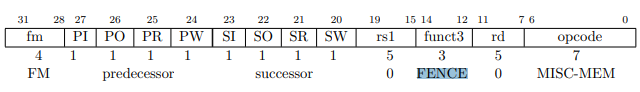
\includegraphics[width=\linewidth]{fence_spec.png}
			\caption{Fence instruction.}
		\end{figure}

		A instrução permite a especificação de qualquer conjunto de \textit{Inputs} (I),
		\textit{Outputs} (O), \textit{Reads} (R) e \textit{Writes} (W) que devam ser
		ordenadas. Essa distinção entre operações de memória (R/W) e de entrada e saída (I/O)
		serve para evitar serialização desnecessária em um \textit{driver} de dispositivo, além
		de permitir outros caminhos que não sejam a memória para controlar coprocessadores ou
		dispositivos de I/O.


%----------------------------------------------------------------------------------------
\graphicspath{ {../img/} }

\section*{VirtIO}

O VirtIO é um protocolo de comunicação entre dispositivos virtuais, criado com o objetivo de definir uma API para unificar drivers e facilitar o uso e configuração desses dispositivos, 
visto que existem diversos sistemas de virtualização diferentes e cada um desses realiza a sua própria implementação.
Para alcançar tais objetivos, o virtIO define uma série de abstrações e estruturas, mas de maneira geral seus principais componentes de funcionamento são 3 (três): 
\emph{device status field}, \emph{feature bits} e uma interface chamada \emph{Virtqueue}.


O \emph{device status field} é uma sequência de bits utilizada pelo dispositivo em conjunto com o sistema operacional para realizar a inicialização do mesmo.
Os bits que podem ser setados nesse campo são: \textbf{ACKNOWLEDGE}, indicando que o dispositivo foi reconhecido, \textbf{DRIVER} para indicar que a inicialização começou, \textbf{DRIVER{\_}OK} e \textbf{FEATURES{\_}OK} para sinalizar que a comunicação está pronta para começar.
Por fim, \textbf{DEVICE{\_}NEEDS{\_}RESET} para indicar uma falha fatal do lado do dispositivo e \textbf{FAILED} pelo lado do sistema operacional.
Já o \emph{feature bits field} é utilizado para comunicar sobre quais features são suportadas pelo dispositivo e entrar em acordo com o sistema operacional sobre quais dessas serão utilizadas. Por exemplo, um dispositivo de interface de rede poderia escolher entre checksumming ou scatter-gather realizar o offload.

Por fim, temos a Virtqueue, uma interface alocada na memória do guest (dispositivo) e que realiza a comunicação entre dois grupos: front-end, onde os pedidos de I/O do processo usuário são realizados e então transferidos para o back-end, que os recebe e então executa as operações utilizando os dispositivos físicos. 

\begin{figure}[t]
  \centering
  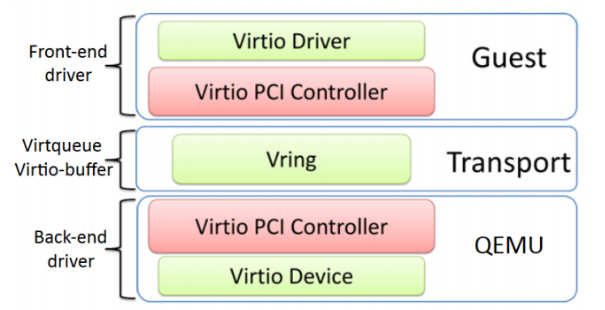
\includegraphics[width=0.85\linewidth]{virtio-arch.png}
  \caption{VirtIO Architecture.}
\end{figure}

\subsection*{Estrutura da Virtqueue}

A Virtqueue é implementada usando uma estrutura chamada \emph{Vring}, que consiste basicamente de 3 (três) partes: um array de descriptors, onde são inseridos os dados,
um \emph{available ring}, usado para a comunicação do sistema operacional com o dispositivo e um \emph{used ring}, utilizado para a comunicação no sentido do dispositivo para o sistema operacional.

Os descriptors contém um endereço físico de 64 bits de buffer junto com o seu tamanho, além de um campo para flags, que podem ser duas: uma para indicar se existe um encadeamento de buffers, permitindo o uso de memória não contígua. 
A outra flag indica o tipo do buffer, se é \emph{read-only} ou \emph{write-only}. Por fim, o campo next aponta para o próximo descriptor, se o mesmo existir. Os outros dois componentes da Virtqueue são chamados de available ring e used ring. O motivo de se utilizar essa estrutura em anéis é permitir assincronicidade, fazendo com que diversas requisições possam ser feitas sem ter que esperar por uma específica finalizar primeiro.

\begin{lstlisting}[language=C]
  struct vring_desc
  {
    __u64 addr;
    __u32 len;
    __u16 flags;
    __u16 next;
  };
\end{lstlisting}


Quando queremos realizar uma ação com o dispositivo, devemos preencher os valores desse descriptor e então adicionar o seu índice dentro de uma lista no available ring.
Dessa forma, ao notificar o sistema operacional, o mesmo irá verificar qual descriptor deve ser lido. A estrutura de um available ring possui seu índice e uma flag, onde é possível desabilitar interrupções, enquanto a constante NUM é negociada entre o dispositivo e o sistema operacional quando o mesmo é inicializado.

\begin{lstlisting}[language=C]
  struct vring_avail
  {
    __u16 ring[NUM];
    __u16 flags;
    __u16 idx;
  };
\end{lstlisting}

Ainda, temos os used rings, onde o dispositivo pode enviar algumas informações ao sistema operacional, como por exemplo indicar que uma operação foi finalizada.
Sua estrutura é muito semelhante a do available ring, com a diferença que aqui o SO tem que procurar qual descriptor realizou a notificação.

\begin{lstlisting}[language=C]
  struct vring_sed
  {
    __u16 flags;
    __u16 idx;
    __u16 avail_event;
    Elem ring[NUM];
  };

  struct Elem {
    u32 id;
    u32 len;
  }
\end{lstlisting}


Outra diferença entre o available e o used ring é que aqui, no used ring, o campo \emph{idx} indica o primeiro elemento não usado do anel.
Isso é utilizado pois dentro da estrutura 'Elem', também temos o índice do descriptor. Assim, a cada leitura realizada, o dispositivo incrementa o índice em used ring.
Dessa forma, se os índices não são iguais, significa que existe ainda dados a serem lidos. 	Tanto o sistema operacional quanto o dispositivo acompanham o estado desses anéis, garantindo que estejam falando sobre a mesma requisição.


Por fim, para indicar onde procurar na memória pelos descriptors, os dispositivos do virtIO tem um registrador chamado \emph{QueuePFN (Page Field Number)} , que contém o endereço de memória física para o qual foi mapeado. Com esse componentes, conseguimos então realizar todo o ciclo de uma requisição. Iniciamos apontando para o endereço de memória existente em QueuePFN e então, quando um descriptor for preenchido com dados, notificamos que uma requisição foi realizada através de um outro registrador, chamado \emph{QueueNotify}, escrevendo um valor qualquer no mesmo. O processo se inicia e quando o mesmo finalizar, uma interrupção externa será enviada pelo dispositivo, de forma que o sistema operacional precisa apenas verificar o used ring e obter os dados.


\subsection*{Exemplo de configuração e uso de um dispositivo}

Para iniciar o processo de uso e configuração de um dispositivo, precisamos começar lendo todo o barramento e procurar pelo chamado \emph{Magic Value}, i.e, a string 'virt'.
Neste exemplo, usando o QEMU, precisamos verificar todos os endereços entre 0x1000{\_}1000 e 0x1000{\_}8000, pois é onde os dispositivos virtios são alocados pelo QEMU.
Encontrado esse valor, podemos ler então o valor do registrador \emph{DeviceID}, que identifica o tipo de dispositivo. Nesse caso, procuramos pelo valor 2, para \emph{block devices}.
O trecho de código abaixo mostra um pedaço dessa leitura de endereços até encontrarmos o dispositivo desejado.

\begin{lstlisting}[language=C]
for addr in (MMIO_VIRTIO_START..=MMIO_VIRTIO_END).step_by(MMIO_VIRTIO_STRIDE) {
  let magicvalue;
  let device_id;
  let ptr = addr as *mut u32;

  unsafe {
    magicvalue = ptr.read_volatile();
    deviceid = ptr.add(2).read_volatile();
  }

  if MMIO_VIRTIO_MAGIC != magicvalue {
    continue;
  }
  else if 0 == deviceid {
    println!("not connected.");
  }
  else {
    match deviceid {
      2 => {
        if false == setup_block_device(ptr) {
          println!("setup failed.");
        }
        else {
          let idx = (addr - MMIO_VIRTIO_START) >> 12;
          unsafe {
            VIRTIO_DEVICES[idx] =
              Some(VirtioDevice::new_with(DeviceTypes::Block));
          }

          println!("setup succeeded!");
        }
      },
      _ => println!("unknown device type."),
    }
  }
}
\end{lstlisting}

Feito isso, começamos a configurar o dispositivo e sua comunicação com o sistema operacional. Iniciamos essa configuração setando o bit de \textbf{ACKNOWLEDGE} no device status, seguido do bit de \textbf{DRIVER}.
Além disso, precisamos entrar em acordo com o dispositivo sobre quais features serão habilitadas, através da leitura do registrador \emph{guest{\_}features} e então setando o bit de \textbf{FEATURES{\_}OK}. 
Por fim, setamos o bit de \textbf{DRIVER{\_}OK} e agora o dispositivo está conectado. O trecho de código abaixo mostra como seria esse processo para um dispositivo genérico.

\begin{lstlisting}[language=C]
  // Reseta o dispositivo e pega o status bit
  ptr.add(MmioOffsets::Status.scale32()).write_volatile(0); 
  let mut status_bits = StatusField::Acknowledge.val32();

  // Seta o ACKNOWLEDGE e o DRIVER no status bit
  ptr.add(MmioOffsets::Status.scale32()).write_volatile(status_bits);
  status_bits |= StatusField::DriverOk.val32();
  ptr.add(MmioOffsets::Status.scale32()).write_volatile(status_bits);

  // Seta o FEATURES{\_}OK no status bit
  status_bits |= StatusField::FeaturesOk.val32();
  ptr.add(MmioOffsets::Status.scale32()).write_volatile(status_bits);

  // Seta o DRIVER{\_}OK no status bit e o dispositivo está conectado
  status_bits |= StatusField::DriverOk.val32();
  ptr.add(MmioOffsets::Status.scale32()).write_volatile(status_bits);
\end{lstlisting}

O VirtIO define uma série de protocolos para cada tipo de dispositivo quando vamos fazer uma requisição, então precisamos seguir o definido para dispositivos do tipo block.
Sendo assim, usaremos 3 (três) descriptors nesse processo: uma para o header, buffer e status.
O do header é responsável por dizer para o dispositivo se o sistema operacional quer escrever ou ler e o endereço onde essa ação deve ocorrer.
O buffer, se for de leitura, irá escrever seu valor na memória, caso seja escrita, o dispositivo irá ler o endereço na memória.
Por fim, o status field guarda o resultado da requisição, que pode ter 3 (três) valores: 0 - success, 1 - failure ou 2 - unsupported operation.


Para realizar a requisição, pegamos os três descriptors que precisamos, inserimos os dados de header, buffer e status e então escrevemos o valor 0 dentro do registrador queue{\_}notify para avisar ao dispositivo que ele deve iniciar a trabalhar na requisição.
Ao finalizar a execução, o dispositivo então emite uma interrupção e recebemos de volta um used ring, o qual contém um id para identificar o descriptor usado. Isto se deve pois as requisições podem 
acabar numa ordem diferente do que foram enviadas, o que faz com que não tenhamos garantia de que é o mesmo descriptor e torna necessário que isso seja checado.
Por fim, validado o descriptor e recebida a resposta, é possível liberar a memória da heap que foi alocada no ínicio da requisição e finalizar a mesma.

\nocite{RISCVUserISA}  % Forces reference
\nocite{virtioPaper}
\nocite{virtioManual}

\bibliographystyle{plain}
\bibliography{references.bib}{}

\end{document}
